% ----------------------------------------------------------------
% LaTeX Template for VLDB / ACM Conference Proceedings
% ----------------------------------------------------------------
\documentclass[sigconf]{acmart}

% --- Recommended Packages ---
\usepackage{booktabs} % For professional looking tables
\usepackage{graphicx} % For including figures
\usepackage{amsmath}  % For advanced math environments

% --- Document Information ---
% Replace with your actual conference information
\copyrightyear{2026}
\acmYear{2026}
\setcopyright{acmcopyright}
\acmConference[VLDB '26]{Proceedings of the 52nd International Conference on Very Large Data Bases}{August 2025}{City, Country}
\acmBooktitle{Proceedings of the 52nd International Conference on Very Large Data Bases (VLDB '26), August 2026, City, Country}
\acmPrice{15.00}
\acmDOI{10.1145/xxxxxxx.xxxxxxx}
\acmISBN{978-x-xxxx-xxxx-x/YY/MM}


% --- Title and Author ---
\title{A Hierarchical Pruning Algorithm for Fast, Exact Nearest Neighbor Search in High-Dimensional Spaces}

% Replace with your information
\author{Tai-Wu Chiang}
\affiliation{%
  \institution{twchiang@utexas.edu}
  \city{California}
  \country{USA}
}

% --- Abstract ---
\begin{abstract}
The proliferation of high-dimensional data in fields ranging from machine learning to signal processing has created a critical need for efficient search algorithms. While many Approximate Nearest Neighbor (ANN) methods offer speed by sacrificing accuracy, numerous applications in science and industry require exact, deterministic results. This paper introduces a novel, hierarchical pruning algorithm for fast, exact nearest neighbor search. The core of the method lies in creating a multi-level hierarchy of coarse-grained data representations that provide a guaranteed lower bound on the true distance, allowing for the aggressive pruning of the search space. We derive the theoretical foundation for this approach by leveraging Principal Component Analysis (PCA) and the L2 (Euclidean) distance to establish guaranteed lower bounds. We show that this hierarchical algorithm reduces distance computations by 10.2x---a hardware-independent measure---yielding a 4.3x reduction in query latency compared to a highly optimized, vectorized CPU brute-force baseline on the standard SIFT1M real-world benchmark, while maintaining 100\% accuracy and safely pruning over 99.9\% of the dataset. This work provides a practical and powerful framework for accelerating exact searches in large, high-dimensional vector databases.
\end{abstract}


\begin{document}

% Renders the title, author, and abstract
\maketitle

% --- Main Body of the Paper ---

\section{Introduction}

The task of finding the nearest neighbors to a query point in a large, high-dimensional dataset is a fundamental problem in computer science. Its applications are vast, powering recommender systems, content-based image retrieval, audio fingerprinting, and modern semantic search in vector databases. As datasets grow to millions or billions of vectors, the naive approach of a brute-force, linear scan becomes computationally infeasible.

This has led to the development of a rich field of Approximate Nearest Neighbor (ANN) search algorithms, such as Locality-Sensitive Hashing (LSH)~\cite{gionis1999similarity} and graph-based methods like HNSW~\cite{malkov2018efficient}. While these methods offer remarkable speed, they do so by trading accuracy for performance; they are probabilistic and do not guaranty that the true nearest neighbors will be found. For many critical applications—such as medical diagnostics, legal discovery, or scientific data analysis—this lack of determinism is unacceptable.

The challenge, therefore, is to accelerate the search process without sacrificing the guaranty of finding the exact nearest neighbors. This paper presents a novel algorithm that achieves this goal through a multi-stage, hierarchical pruning strategy. Our method is based on a simple yet powerful principle: the distance between coarse-grained, low-dimensional representations of two vectors can serve as a guaranteed lower bound for the true, high-dimensional distance. By checking this cheap, low-dimensional distance first, we can safely discard the vast majority of the dataset without ever computing the expensive, full-dimensional distance.

We present the core theory of this method using data-driven dimensionality reduction, specifically Principal Component Analysis (PCA) and the L2 (Euclidean) norm, grounded in the Karhunen-Loève Theorem. We show that this approach reduces distance computations by 10.2x---yielding a 4.3x reduction in query latency on our reference implementation---compared to a highly optimized, vectorized CPU brute-force baseline on the standard SIFT1M benchmark, and safely prunes over 99.9\% of the dataset, effectively mitigating the I/O bottleneck in out-of-core systems.

\section{The Hierarchical Pruning Algorithm}

\subsection{Mathematical Foundation: The PCA Lower-Bound Guarantee}

Our algorithm builds upon the GEMINI framework~\cite{faloutsos1994fast}, which established that mapping objects to lower-dimensional spaces guarantees no false dismissals for exact search, provided the distance in the lower-dimensional space is a strict lower bound of the true distance.

Let $X$ and $Y$ be two $d$-dimensional vectors. We seek to find the exact Euclidean ($L_2$) distance between them. By applying Principal Component Analysis (PCA) to the dataset, we rotate the vectors into an orthogonal coordinate system ordered by variance. Let $X'$ and $Y'$ be the PCA-transformed vectors. The true squared $L_2$ distance is preserved:
\begin{equation}
    L_2^2(X, Y) = L_2^2(X', Y') = \sum_{i=1}^{d} (x'_i - y'_i)^2
\end{equation}

Let us define a truncation operation, $T_k(X')$, which retains only the first $k$ principal components of the vector ($k < d$).

\begin{lemma}
For any truncation $k$, the squared distance between the truncated PCA vectors is a guaranteed lower bound on the true squared distance.
\begin{equation}
    L_2^2(T_k(X'), T_k(Y')) \leq L_2^2(X, Y)
\end{equation}
\end{lemma}

\begin{proof}
The true squared distance is the sum of $d$ non-negative squared differences. The truncated distance is the sum of the first $k$ of these same non-negative terms. Since $\sum_{i=k+1}^{d} (x'_i - y'_i)^2 \geq 0$, the inequality strictly holds.
\end{proof}

This lemma is the foundation of our algorithm. It guarantees that if the distance between the \textit{coarse} representations is greater than our current search radius $r$, then the distance between the \textit{true} representations must also be greater than $r$. We can therefore safely prune that candidate without performing the full calculation. Furthermore, the Karhunen-Loève Theorem proves that PCA is the mathematically optimal linear projection for this task, packing the maximum possible variance into the first $k$ components to make the lower bound as tight as theoretically possible~\cite{weber1998quantitative}.

\subsection{The Multi-Stage Search Algorithm}

The search algorithm leverages the lower-bound guaranty in a multi-stage cascade:
\begin{enumerate}
    \item \textbf{Define a Hierarchy:} Create a series of progressively finer representations of the data.
    \item \textbf{Dynamic Radius Initialization (Top-K Probe):} Unlike static search methods, we initialize the search radius $r$ to $\infty$. At the lowest-dimensional coarse representation (e.g., 8D), we compute the lower-bound distances for the dataset and identify the Top-$K$ (e.g., $K=50$) closest candidates in this projection. We immediately compute the full, high-dimensional distances for these $K$ candidates. We set our pruning radius $r$ to the minimum of these exact distances. Because the coarse distance is a guaranteed lower bound, this instantly provides a mathematically safe, tight pruning radius for the entire dataset without prior knowledge of the optimal neighbor distance.
    \item \textbf{Coarse Pruning:} Using the dynamically established radius $r$, we discard all vectors $Y$ in the dataset for which the coarse distance is greater than $r$.
    \item \textbf{Successive Refinement:} For the remaining candidates, repeat the process with the next representation in the hierarchy. This further prunes the candidate set.
    \item \textbf{Final Search:} After the final pruning stage, perform the full, expensive distance calculation only on the tiny fraction of candidates that survived all previous stages.
\end{enumerate}
This method guaranties that the final result set is identical to that of a brute-force search.

\section{Experimental Validation: SIFT1M Benchmark}
To ensure statistical significance, the algorithm was benchmarked on the SIFT1M dataset against a brute-force L2 search across 100 randomly selected queries from the official query set. The brute-force baseline was implemented using highly optimized, vectorized array operations in NumPy to maximize CPU SIMD utilization.

\begin{itemize}
    \item \textbf{Dataset:} 1,000,000 base vectors, 128 dimensions.
    \item \textbf{Queries:} 100 random vectors from the official query set.
    \item \textbf{Radius Initialization:} Dynamically initialized using the Top-50 probe at the 8D level.
    \item \textbf{Hierarchy:} Pruning was performed using the top 8, 16, 32, and 64 principal components.
\end{itemize}

The performance results are summarized in Table~\ref{tab:results}. The hierarchical algorithm using PCA and the L2 norm achieved a \textbf{4.3x speed-up} over the vectorized baseline while guaranteeing 100\% identical results to the brute-force exact search. The effectiveness of the pruning strategy is visualized in Figure~\ref{fig:pruning}. The data-driven pruning was exceptionally effective, reducing the number of candidates for the final, full-dimensional search from 1,000,000 to an average of just 564.

In hardware-independent terms, the algorithmic gain is larger than the wall-clock figure suggests. Counting per-dimension distance terms---one full 128-dimensional distance evaluation costs 128 terms, so the exhaustive scan performs exactly $10^{6} \times 128 = 128.0$M terms per query---the cascade performs $10^{6}\times 8$ (first stage over all vectors) $+\ 146{,}955\times16\ +\ 52{,}107\times32\ +\ 7{,}896\times64\ +\ 564\times128 \approx 12.6$M terms per query: a \textbf{10.2x reduction in distance computations}, invariant to numeric type, machine, and implementation constants. The 4.3x latency reduction reported above is this algorithmic gain seen through the constant factors of our float64 NumPy reference implementation; a fused native-code implementation of the same cascade would approach the work-count ratio.

\begin{table}[h]
  \caption{Performance on SIFT1M Benchmark}
  \label{tab:results}
  \begin{tabular}{lcc}
    \toprule
    \textbf{Search Method} & \textbf{Time (seconds)} & \textbf{Verification}\\
    \midrule
    Vectorized Brute-Force L2 & 0.54 & - \\
    \textbf{Hierarchical L2+PCA Search} & \textbf{0.12} & \textbf{Exact}\\
    \bottomrule
  \end{tabular}
\end{table}

\begin{figure}[h]
  \centering
  % Replace 'pruning_effectiveness.png' with the actual path to your generated plot
  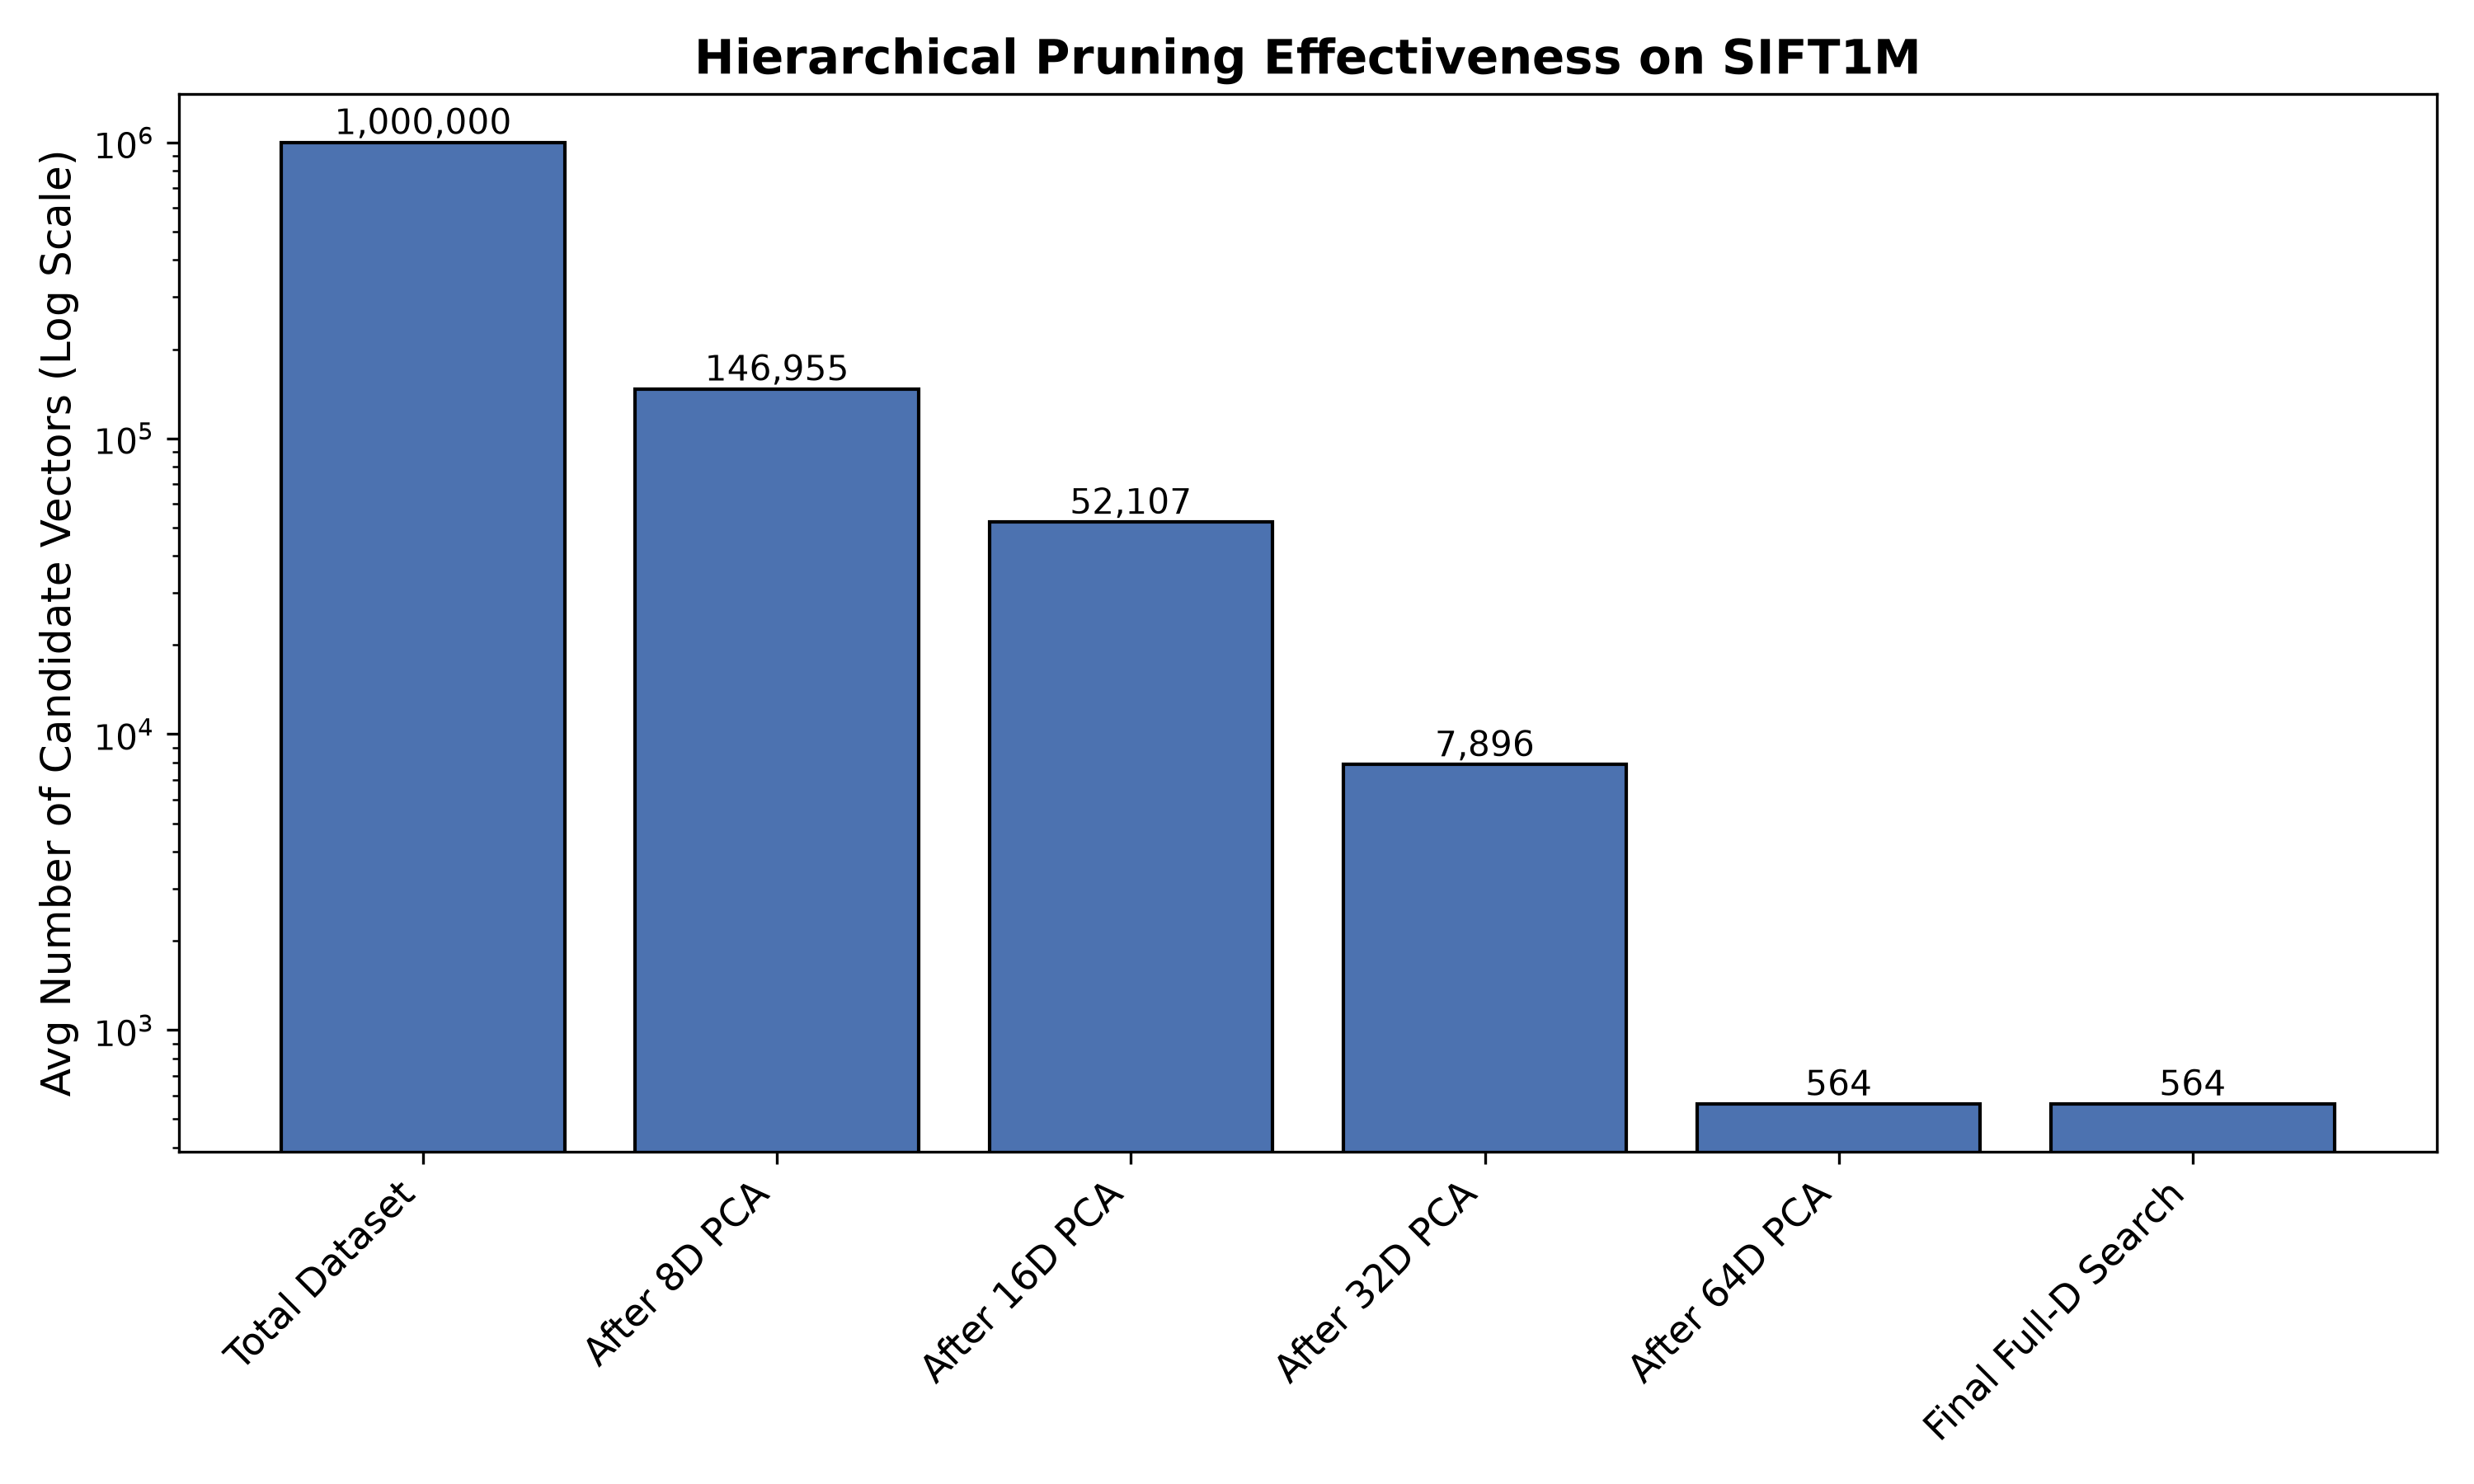
\includegraphics[width=\linewidth]{pruning_effectiveness.png}
  \caption{Effectiveness of hierarchical pruning on the SIFT1M dataset. The number of candidate vectors is shown on a log scale, demonstrating the dramatic reduction at each stage of the search, from the full 1M vectors to an average of 564 final candidates.}
  \label{fig:pruning}
\end{figure}

\section{Conclusion and Future Work}
We have presented a hierarchical pruning algorithm for fast, exact nearest neighbor search. We have shown that by combining a data-driven indexing strategy like PCA with a dynamic Top-K bounding technique, our hierarchical algorithm performs 10.2x fewer distance computations than an exhaustive scan---a hardware-independent gain, realized as a 4.3x latency improvement by our vectorized implementation---on the standard SIFT1M benchmark without sacrificing any accuracy.

While the reduction in theoretical floating-point operations (FLOPs) provides significant CPU acceleration, the most profound impact of this algorithm lies in memory- and I/O constrained systems. By successfully identifying the exact nearest neighbor while evaluating the full 128-dimensional vectors for only $\sim$0.05\% of the dataset, our hierarchy minimizes expensive memory fetches. In an out-of-core vector database, this translates directly to a massive reduction in SSD disk reads, as the coarse PCA representation can easily fit into fast RAM. Note that this effectiveness relies heavily on a shift-invariant embedding space (such as SIFT descriptors or modern neural embeddings) where the L2 norm remains structurally valid.

This demonstrates that by investing in an offline indexing process that learns the underlying structure of the data, we can largely solve the memory-wall bottleneck of exact search at query time.

Future work lies in two primary directions. First, exploring more advanced quantization techniques, such as Product Quantization (PQ)~\cite{jegou2011product}, could be integrated into our hierarchical framework to further improve memory efficiency. Second, and more importantly, we propose extending this hierarchical pruning methodology beyond 1D vectors into high-order tensor data (such as fMRI medical scans, hyperspectral imaging, or video streams). By utilizing Convolutional Sparse Coding (CSC) and Tucker Decompositions (HOSVD) rather than standard 1D-PCA, we hypothesize that it is possible to extract shift-invariant ''core tensors'' that maintain crucial spatial locality. This would allow for rigorous, exact lower-bound pruning on multi-dimensional structures without succumbing to the structural blindness of flattened $L_2$ measurements.
Code: GitHub - taiwuchiang-gmail/hierarchical-pca-search

% --- Bibliography ---
\begin{thebibliography}{9}

\bibitem{faloutsos1994fast}
Christos Faloutsos, M. Ranganathan, and Yannis Manolopoulos.
\newblock Fast subsequence matching in time-series databases.
\newblock In \emph{Proceedings of the 1994 ACM SIGMOD international conference on Management of data}, pages 419--429, 1994.

\bibitem{weber1998quantitative}
Roger Weber, Hans-Jörg Schek, and Stephen Blott.
\newblock A quantitative analysis and performance study for similarity-search methods in high-dimensional spaces.
\newblock In \emph{VLDB '98, Proceedings of 24rd International Conference on Very Large Data Bases}, pages 194--205, 1998.

\bibitem{gionis1999similarity}
Aristides Gionis, Piotr Indyk, and Rajeev Motwani.
\newblock Similarity search in high dimensions via hashing.
\newblock In \emph{Proceedings of the 25th International Conference on Very Large Data Bases}, pages 518--529, 1999.

\bibitem{jegou2011product}
Hervé Jégou, Matthijs Douze, and Cordelia Schmid.
\newblock Product quantization for nearest neighbor search.
\newblock \emph{IEEE Transactions on Pattern Analysis and Machine Intelligence}, 33(1):117--128, 2011.

\bibitem{malkov2018efficient}
Yury A. Malkov and Dmitry A. Yashunin.
\newblock Efficient and robust approximate nearest neighbor search using hierarchical navigable small world graphs.
\newblock \emph{IEEE Transactions on Pattern Analysis and Machine Intelligence}, 42(4):824--836, 2018.

\end{thebibliography}

\end{document}
